\chapter{Evaluering av brukertestene}
Som nevnt i \ref{brukertest} ble det utformet en plan for brukertestene, både for å være mest mulig forberedt og for å utvikle en brukertest som lignet reelle situasjoner der applikasjonen ville bli brukt. I tillegg gjennomførte utviklerne brukertesten selv flere ganger for å undersøke om den var godt utformet og for å avdekke eventuelle kritiske problemområder eller feil i applikasjonen. Her vil det skilles mellom et problem og en feil i applikasjonen. Med problemer menes funksjonalitet eller designvalg i applikasjonen som hindrer eller forvirrer i sånn måte at brukeren ikke klarer å bruke applikasjonen som tiltenkt. Feil vil regnes som programvarefeil i koden som gi diverse uheldige konsekvenser for applikasjonen. For å evaluere brukertestene tas det utgangspunkt i resultattabellen som var presentert i \ref{resultattabell}. Fra tabellen vil problemene bli kategorisert i kritiske, alvorlige og mindre problemer som beskrevet av analyse -og markedsføringselskapet Hotjar \cite{HotjarWebsiteHeatmaps}. I følge dem kategoriseres problemene som oppdages i brukertestene slik \cite{HowAnalyzeEvaluate2020}: 
\begin{itemize}
    \item \textbf{Kritiske problemer:} Umulig for brukerne å fullføre oppgaver.
    \item \textbf{Alvorlige problemer:} Frustrerende for mange brukere.
    \item \textbf{Mindre problemer:} Irriterende problem, men ikke nok til å drive vekk brukere. 
\end{itemize}

\section{Kritiske problemer} \label{kritiske_feil}
Det ble oppdaget en kritisk feil ved første brukertest der testdeltakeren ikke klarte å laste opp informasjonen som var hentet inn om oppsynsturen opp til databasen i Cloud Firestore. Ettersom brukertestene var kvalitative, ble det improvisert en falsk oppsynstur som deltakeren kunne laste opp slik at siste oppgave som var å sjekke den nylige opplastede oppsynsturen. De resterende brukertestene ble satt på vent til feilen ble fikset. Denne feilen viste seg å være på grunn av at oppsynsturen ble for stor til å lagres i Firestore når bildet som ble tatt under oppgave 5 ble lagret som en base64-streng.
\newline
\newline
Grunnet tilfeldigheter knyttet til størrelsen på bildene tatt i applikasjonen og informasjonen som ble lagret fra oppsynstur ble ikke denne feilen oppdaget under intern testing mens utviklingen foregikk. Det ble forsøkt med å skru ned bildekvaliteten slik at oppsynsturen kunne lastes opp i databasen, men resultatet ble fortsatt ikke stabilt nok. Det ble derfor bestemt å endre brukertestene slik at bildet fjernes før oppsynsturen lagres i databasen slik at brukertestene kunne gjennomføres som planlagt. I tillegg gjorde denne tilnærmingen at funksjonaliteten for å fjerne bilder ble testet, noe som ikke var en del av den opprinnelige brukertesten. 
\newline
\newline
Denne feilen kan rettes opp på flere måter. Et av alternativene er å bruke Firebase sitt Cloud Storage-funksjonalitet \cite{CloudStorageFirebase2021}. Cloud Storage gjør det mulig å lagre filer i skyen direkte fra applikasjonen. Selv ved dårlig nettverksforbindelse ved ned- og opplasting av filer vil applikasjonen få mulighet til å prøve å sende eller hente filene nytt idet nettverksforbindelsen returnerer \cite{CloudStorageFirebase2021}. Med tanke på at prosjektet allerede benytter seg av Firebase Authentication og Cloud Firestore, er dette det beste alternativet for opp- og nedlasting av bilder i prosjektet.

\section{Alvorlige problemer}
Det ble også avdekket alvorlige problemer som hindre applikasjonen til å være like effektiv og behjelpelig for brukerne som tiltenkt. Et av problemene som gikk igjen flest ganger blant testdeltakerne var at de ikke forstod at markøren på kartet viste lokasjonen der registrerte observasjoner ville visualiseres på kartet med en pin, og at kartet derfor burde flyttes på før en ny registrering. Noen av deltakerne oppdaget dette selv etter å ha registrert en observasjon og deretter oppdaget at det ble opprettet en pin der, men flere måtte få hjelp av forsøkslederen for å forstå hvordan dette foregikk. Selv om dette problemet ikke nødvendigvis frustrerte deltakerne ettersom de ikke var klar over problemet, men det kan potensielt bli svært frustrerende i ettertid når observasjonene ikke blir plassert på faktisk lokasjon, særlig når koordinatene skal sendes til myndighetene. Dette kan løses med å forklare bruken av markøren med en demonstrasjonvideo eller animasjon første gangen brukeren benytter seg av applikasjonen samt finne et mer passende ikon enn hårkors-ikonet som ble implementert. I tillegg kan det legges til en vindu som kommer opp med med beskrivende tekst når markøren trykkes på dersom brukerne blir usikre på hvordan markøren brukes. Slike vindu tilbys allerede i Leaflet-biblioteket som benyttes for kartet.
\newline
\newline
Et annen alvorlige problem som oppstod for én av deltakerne var at GPS-posisjonen ble unøyaktig og hoppet på kartet før den fant riktig posisjon, som både førte til forvirring for deltakeren og at GPS-ruten for oppsynsturen ble unøyaktig. Dette problemet skyldtes at GPS-signalet rekalibrerte seg dersom applikasjonen gikk i dvale eller ble lukket og dermed ville den første koordinaten ofte være unøyaktig. Ettersom det ble for utfordrende å kontinuerlig hente lokasjonen i bakgrunnen, ble problemet løst ved å legge til strømsparingsmodus slik at det ikke var nødvendig å gå ut av applikasjonen og en algoritme som tok seg av en ekstra rekalibrering når applikasjonen ble aktiv igjen. Denne algoritmen sammenligner hvor lang tid det går mellom hver registrering av et nytt koordinat og avstanden på koordinatene slik at applikasjonen vil ignorere koordinater som tilsier at personen har bevegd seg i hastigheter lang over rask gange.
\newline
\newline
Et alvorlig problem som var forutsett og forventet av utviklerne, var at deltakerne som ikke var kjente med registreringsgrensesnittet ville slite med å forstå sveiping-bevegelsene i begynnelsen. Utviklerne ønsket å se hvor vanskelig det var å forstå grensesnittet uten hjelp, og som forventet slet begge deltakerene markant mer enn deltakerne som hadde fått vist registreringsgrensesnittet tidligere. En av deltakerne måtte få hjelp for å kunne gå videre i brukertesten. Det har lenge vært en tanke å legge til en demonstrasjon av hvordan registreringsgrensesnittet brukes i blinde, enten med en video eller animasjon som vises første gang applikasjonen brukes slik at nye brukere får en innføring i hvordan brukergrensesnittet brukes med sveiping og annet funksjonalitet. Brukertestene viser at dette er essensielt for at brukerene skal kunne utnytte registreringsfunksjonaliteten på best mulig vis slik at applikasjonen blir et hjelpsomt verktøy. 
\newline
\newline
En av testdeltakerne fikk problemer med å opprette og lagre et nytt øremerke i registreringsgrensesnittet. Når brukerne skriver navnet på personen som øremerket skal registreres på i tekstfeltet, presser mobiltastaturet navigasjonsknappene nederst på siden lengre opp slik at disse knappene kommer nært \enquote{Lagre}-knappen (se figur \ref{fig:oremerke_feil} under). Dette førte til at deltakeren kom borti \enquote{Neste}-knappen under og applikasjonen gikk dermed videre i registreringen uten at det øremerket ble lagret. Deltakeren måtte gå tilbake til siden for øremerker og registrere på nytt, som var et irritasjonsmoment for deltakeren. Problemet kan rettes på ved at tastaturet bare legges over navigasjonsknappene uten at de presses opp, slik at deltakeren aktivt må trykke vekk tastaturet for å bruke \enquote{Neste}-knappen.  
\begin{figure}[H]
\centering
\captionsetup{width=.8\linewidth}
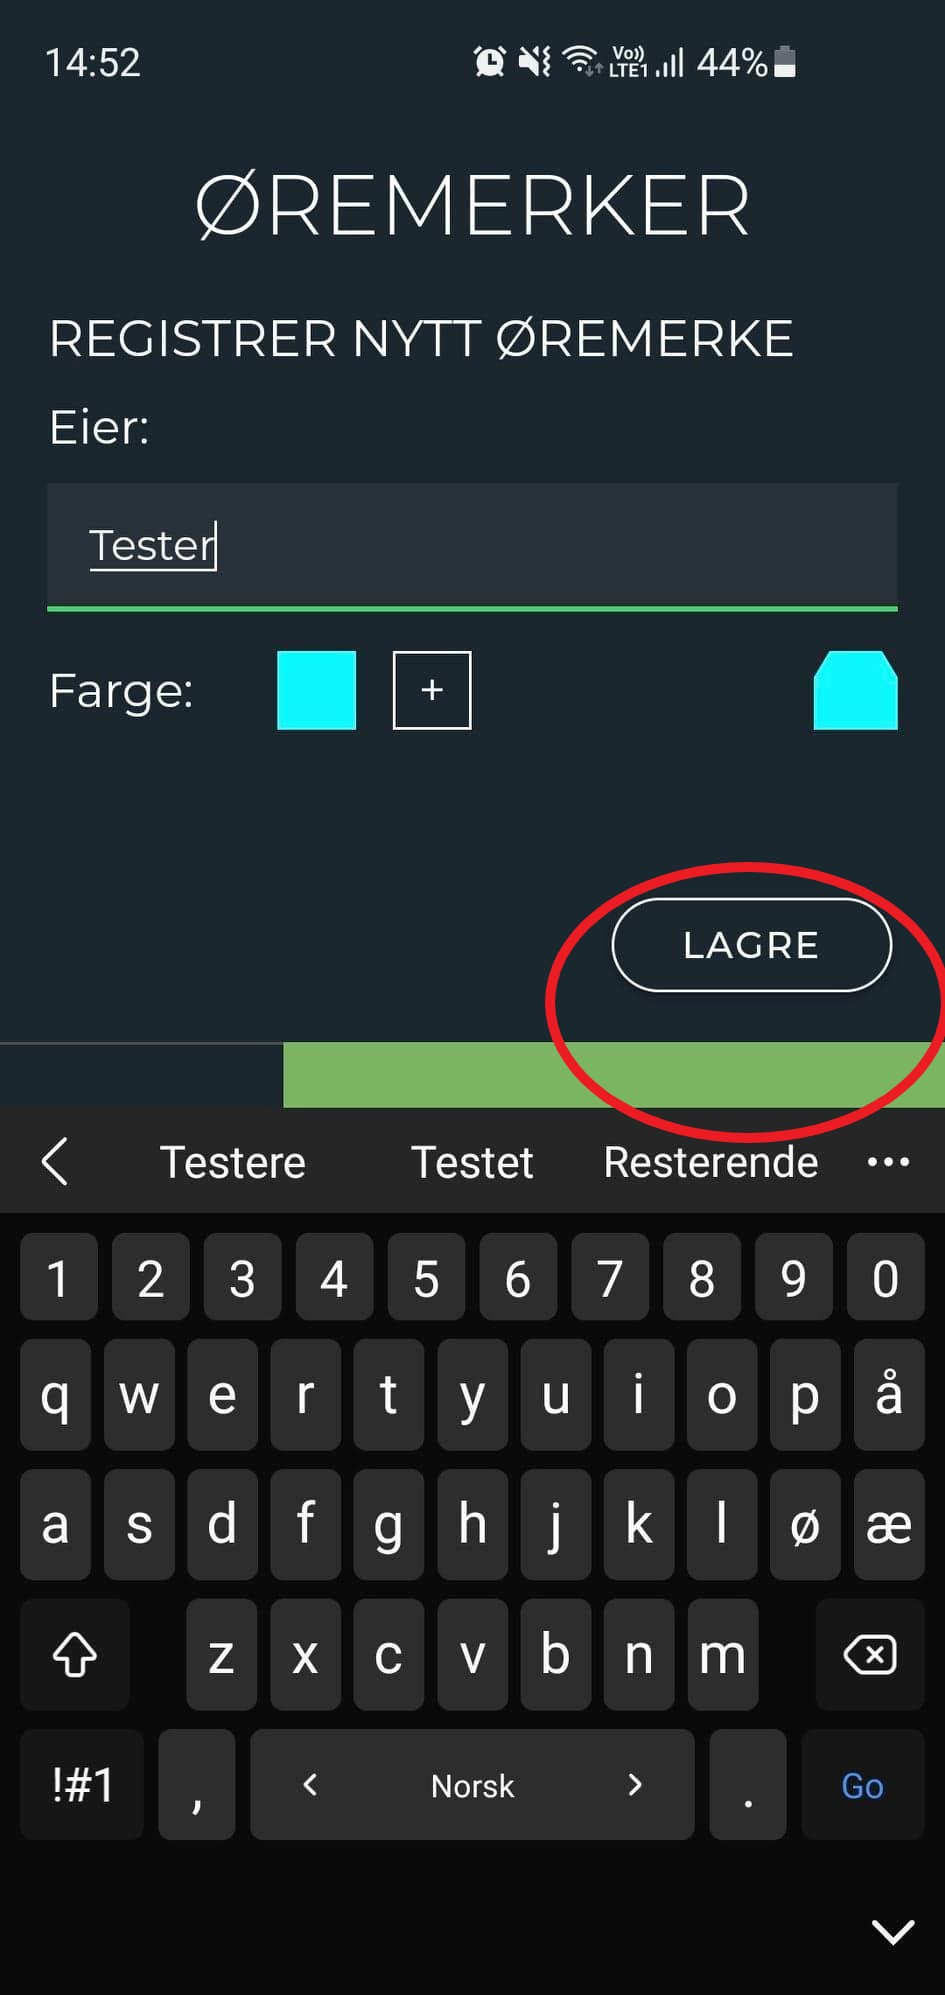
\includegraphics[scale=0.3]{Figurer/skjermbilder/oremerke_feil.jpg}
\caption{Figur som viser hvordan tastaturet skyver opp navigasjonsknappene til \enquote{Lagre}-knappen i siden for registrering av øremerker.}
\label{fig:oremerke_feil}
\end{figure}

\section{Mindre problemer}
Et par mindre problemer ble oppdaget i brukertestene. Et av problemene som oppstod flest ganger blant testdeltakerne var at brukerne i siden for oppsynsturer trykket på hele boksen for å gå inn på en spesifikk oppsynstur og ikke pilen til høyre. Siden hver oppsynstur er fremhevet som bokser med en farget kant rundt, er det naturlig å tro at hele boksen skal trykkes på. Det er i tillegg enklere å trykke på boksen enn pilen med tanke på at boksen har større flate, så hele boksen bør implementeres til å være trykkbar slik de fleste brukerne ønsket. 
\newline
\newline
En deltaker krysset ikke av for det øremerket som personen akkurat hadde opprettet og gikk dermed videre til oppsummeringssiden der øremerket ikke var registrert. Dette viser at brukerne antar at når det opprettes og lagres et nytt øremerke, så forventes det at dette øremerket da automatisk blir krysset av. 
To av testdeltakerne trykket på bildeikonet og ikke \enquote{Pluss}-knappen for å ta bilde i siden for registrering av død sau. For å unngå forvirring og at andre brukere støter på samme problem, kan bildeikonet enten gjøres mindre enn det er nå eller fjernes helt.  
\newline
\newline
En av deltakerne tok feil av plaster- og dødningshodeikonet da personen skulle registrere en død sau. Personen oppdaget raskt at plasterikonet var for skadet sau og gikk videre til dødningshodet etterpå. Selv om dette var et enkelttilfelle blant deltakerene i brukertesten og resten forstod betydningen av ikonene på første forsøk, kan det være viktig å presisere ikonene slik at flere brukere ikke møter på dette problemet. Beskrivelse av ikonene kan også legges inn i demonstrasjonen av applikasjonens funksjoner som er nevnt tidligere, slik at brukerne får en bekreftelse på hva ikonene representerer. Videre kan det gjennomføres A/B-testing der man viser to grupper av brukere ulike versjoner av ikonene og deretter sammenligner versjonene for å se hvilken som ble best mottatt av brukerne. 